\section{Fresnel lollipops - separation error}

The phase and amplitude of the scattered signal are extracted using traditional signal processing techniques.
The end result is a single value in the two dimensional IQ plane.
In the absence of noise, the two possible qubit states would correspond to two individual IQ points as indicated by the black dots in Fig.\,\ref{Fig:lollipop}.
In this case, any nonzero separation between the points would allow distinction between the qubit states.
However, in the real system, both technical and quantum noise add statistical fluctuations to the extracted IQ points.
The ``quantum noise'' is just the intrinsic width of the wave functions of the coherent microwave pulse, which carries a noise power of $\hbar \omega / 2$ per unit bandwidth.
A minimum additional $\hbar \omega / 2$ of quantum noise is added by a phase preserving parametric amplifier \cite{Caves:amplifiers1982}.
Technical noise may be added by following amplifiers, such as a HEMT.
Signal loss prior to the dominant amplifier stages also appears as effective added noise.

\begin{figure}
\begin{centering}
\includegraphics[width=8cm]{lollipop.pdf} 
\par\end{centering}
\caption{IQ clouds for the qubit states measured in the presence of noise. The clouds for $\ket{0}$ (blue) and $\ket{1}$ (red) are centered on the diametrically opposite points of the $S_{21}$ circle. The black dots represent the points which would be found in the absence of all noise sources. The Gaussian curves show projections of the clouds onto the line connecting their centers.}
\label{Fig:lollipop}
\end{figure}

The time domain noise leads to noise in the demodulated IQ points.
Instead of single points corresponding to the two qubit states, we get two-dimensional Gaussian statistical distributions, as shown by the blue and red clouds in Fig.\,\ref{Fig:lollipop} (see Ref. \cite{Schoukens:DFTNoise1986} and \citeinternaltype \citeinternalref{whiteNoiseDFT}).
These clouds have been called ``Fresnel lollipops''.
Projecting the lollipops onto a line separating their centers produces a pair of one dimensional Gaussian curves.
Choosing the center of the curves as the discrimination between $\ket{0}$ and $\ket{1}$, we can see that, because of the finite width $\sigma$ of the curves, there will always be a nonzero probability of misidentifying the qubit state.
We call this error, due to the finite separation of the curves, the ``separation error'', denoted $\epsilon_{\text{sep}}$.
The separation error is computed by integrating the weight of one of the Gaussian distributions which is on the ``wrong'' side of the discrimination point, \begin{eqnarray}
\epsilon_{\text{sep}} &=& \frac{1}{\sqrt{2\pi \sigma^2}} \int_{x=(x_0 + x_1)/2}^{\infty} e^{\frac{-(x-x_1)^2}{2\sigma^2}} \, dx \nonumber \\
&=& \frac{1}{2}\textrm{erfc}\left[ \frac{\left| x_0 - x_1 \right|}{2 \sqrt{2 \sigma^2}} \right] , \label{eq:sec:Lollipops:epsilon_sep} \end{eqnarray}
where the $\textrm{erfc}$ function is defined as \begin{equation}
\textrm{erfc}(z) \equiv 1 - \frac{2}{\sqrt{\pi}}\int_0^z e^{-x^2}\,dx . \end{equation}

Defining the signal to noise ratio (SNR) of the measurement as \begin{equation}
\text{SNR} \equiv \frac{(x_0-x_1)^2}{2 \sigma^2} , \label{eq:sec:lollipops:SNR} \end{equation}
we relate $\epsilon_{\text{sep}}$ to the SNR, \begin{equation}
\epsilon_{\text{sep}} = \frac{1}{2} \textrm{erfc} \left[ \frac{\sqrt{\text{SNR}}}{2} \right] . \label{eq:sec:lollipops:e_sepVsSNR} \end{equation}
